\documentclass[a4paper, 14pt]{extarticle}

\usepackage{newtxtext}
\usepackage[utf8]{inputenc}
\usepackage[T2A]{fontenc}
\usepackage[russian]{babel}

\usepackage[left = 30 mm, right = 10 mm, top = 20 mm, bottom = 20 mm]{geometry}
\usepackage{setspace} \onehalfspacing
\usepackage{indentfirst} \setlength{\parindent}{1.25cm}
\usepackage[autostyle]{csquotes}

\usepackage{fancyhdr} \pagestyle{fancy} \fancyhf{}
\fancyfoot[C]{\thepage} \renewcommand{\headrulewidth}{0pt}

\usepackage{titlesec}
\titleformat{\section}[block]{\centering}{}{0em}{\MakeUppercase}

\usepackage{caption}
\captionsetup[table]{font=small,labelsep=period,skip=10pt,justification=centering}
\captionsetup[figure]{font=small,labelsep=period,skip=10pt,justification=centering}

\usepackage{titletoc}
\titlecontents{section}[0pt]{}{\MakeUppercase}{}{\titlerule*[0.5em]{.}\contentspage}

\usepackage{graphicx, amsmath, array, float, booktabs}
\usepackage[none]{hyphenat} \sloppy

\begin{document}

    \begin{titlepage}
        \begin{center}
            Министерство науки и высшего образования Российской Федерации \\
            Федеральное государственное автономное образовательное учреждение \\
            высшего образования \\
            \enquote{Казанский (Приволжский) федеральный университет} \\
            Институт вычислительной математики и информационных технологий \\
            Кафедра прикладной математики и искусственного интеллекта \\
            \vspace{5 cm}
            ОТЧЕТ \\
            по дисциплине \enquote{Численные методы} \\
            Тема: \enquote{Вычисление интеграла квадратурными формулами} \\
            Вариант 8 \\
            \vspace{3 cm}
        \end{center}
        \begin{flushright}
            Выполнил: студент гр. 09-321, \\
            Лещенко Е.Ф. \\
            Проверил: старший преподаватель \\
            Глазырина О.В. \\
        \end{flushright}
        \vfill
        \begin{center}
            Казань, 2025
        \end{center}
    \end{titlepage}

    \setcounter{page}{2}
    \tableofcontents
    \newpage


    \section{Постановка задачи}\label{sec:-2}
    В математической физике нередко применяется функция ошибки $\mathrm{erf}$:
    \begin{equation}
        \label{eq:definition_erf} \mathrm{erf}(x) = \frac{2}{\sqrt{\pi}} \int\limits_0^x e^{-t^2}dt.
    \end{equation}

    В виде цели работы поставлена реализация различных квадратурных
    форм и сравнение их эффективность.

    Сначала функция~\eqref{eq:definition_erf} раскладывается в ряд Тейлора в окрестности $x = 0$.
    Это позволяет приближённо вычислять значения на отрезке $[a, b]$ с точностью $\varepsilon$,
    которые станут эталонными для оценки других методов.
    Далее интеграл вычисляется численно с помощью пяти квадратур:
    \begin{enumerate}
        \item Метод левых прямоугольников~\ref{subsec:left};
        \item Метод центральных прямоугольников~\ref{subsec:center};
        \item Метод трапеций~\ref{subsec:trapezoid};
        \item Метод Симпсона~\ref{subsec:simpson};
        \item Метод Гаусса~\ref{subsec:gaussian}.
    \end{enumerate}

    Для каждого метода анализируется, как точность зависит от числа разбиений $N$.
    Сравнение проводится по разности между приближённым значением $I_N$ и $I_0$ из ряда Тейлора
    --- будем считать его эталонным.
    Результаты сводятся в таблицу, где для каждого $x_i \in [a, b]$ указаны:
    $I_0$, $I_N$, абсолютная погрешность $|I_0 - I_N|$ и минимальное $N$ для заданной точности.

    В завершение методы сравниваются по точности для выявления наиболее эффективного метода.\newpage


    \section{Ход работы}\label{sec:-}
    Разложим функцию~\eqref{eq:definition_erf} в ряд Тейлора в окрестности нуля.
    Разложение экспоненциальной функции имеет вид:
    $$ e^x = \sum\limits_{n=0}^{\infty} \frac{x^n}{n!}. $$
    Пусть $x = e^{-t^2}.$ Тогда:
    $$ e^{-t^2} = \sum\limits_{n=0}^{\infty} \frac{(-t^2)^n}{n!} = \sum\limits_{n=0}^{\infty} (-1)^n \frac{t^{2n}}{n!}. $$
    Проинтегрируем полученный ряд на отрезке от~$0$ до~$x$:
    $$ \int\limits_0^x \sum\limits_{n=0}^{\infty} (-1)^n \frac{t^{2n}}{n!} dt = \sum\limits_{n=0}^{\infty} (-1)^n \frac{1}{n!} \int\limits_0^x t^{2n}dt = \sum\limits_{n=0}^{\infty} (-1)^n \frac{x^{2n+1}}{n!(2n+1)}. $$
    Таким образом, разложение функции~\eqref{eq:definition_erf} в ряд Тейлора в окрестности нуля имеет вид:
    \begin{equation}
        \label{eq:Taylor_erf}
        \mathrm{erf}(x) = \frac{2}{\sqrt{\pi}} \sum\limits_{n=0}^{\infty} (-1)^n \frac{x^{2n+1}}{n!(2n+1)}.
    \end{equation}

    Для перехода к численному интегрированию для начала
    вычислим функцию~\eqref{eq:definition_erf} в одиннадцати узлах на отрезке~$[0,2]$ с точностью~$\varepsilon = 10^{-6}$.
    Будем использовать равноудаленные узлы, поэтому~$h=0.2$.

    \subsection{Метод левых прямоугольников}\label{subsec:left}
    Используем составную квадратурную формулу левых прямоугольников:
    \begin{equation}
        \label{eq:Quadrature_Formula_Left_Rectangles}
        I_{N} = h \sum\limits_{i=1}^{N - 1} f(x_i).
    \end{equation}
    Вычислим значения функции~\eqref{eq:definition_erf} с помощью разложения в ряд Тейлора~\eqref{eq:Taylor_erf}
    и сопоставим их с полученными результатами.
    Результаты занесены в таблицу~\ref{tab:Left_Rectangles}.
    Возьмем в~\eqref{eq:Quadrature_Formula_Left_Rectangles} количество разбиений~$N=6$.
    График изображен на рис.~\ref{fig:Left_Rectangles}.
    \begin{table}[H]
        \centering
        \begin{tabular}{|c|c|c|c|c|}
            \hline
            $x$  & $J_0(x)$ & $J_n(x)$ & $J_0(x)-J_n(x)$        & $n$     \\ \hline
            0.00 & 0.000000 & 0.000000 & 0                      & 1       \\ \hline
            0.20 & 0.222703 & 0.222703 & $5.42728\times10^{-7}$ & 8192    \\ \hline
            0.40 & 0.428392 & 0.428393 & $5.0994\times10^{-7}$  & 65536   \\ \hline
            0.60 & 0.603856 & 0.603857 & $7.74047\times10^{-7}$ & 131072  \\ \hline
            0.80 & 0.742101 & 0.742102 & $8.48733\times10^{-7}$ & 262144  \\ \hline
            1.00 & 0.842701 & 0.842701 & $6.93895\times10^{-7}$ & 524288  \\ \hline
            1.20 & 0.910314 & 0.910315 & $9.12102\times10^{-7}$ & 524288  \\ \hline
            1.40 & 0.952285 & 0.952286 & $5.94847\times10^{-7}$ & 1048576 \\ \hline
            1.60 & 0.976348 & 0.976349 & $7.42921\times10^{-7}$ & 1048576 \\ \hline
            1.80 & 0.989091 & 0.989091 & $8.64023\times10^{-7}$ & 1048576 \\ \hline
            2.00 & 0.995322 & 0.995323 & $4.18471\times10^{-7}$ & 2097152 \\ \hline
        \end{tabular}
        \caption{Результаты вычислений составной квадратурной формулой левых прямоугольников.}
        \label{tab:Left_Rectangles}
    \end{table}

    Как видно по таблице, в некоторых точках нам понадобилось производить целых~$2\,097\,152$ разбиений.

    \begin{figure}[H]
        \centering
        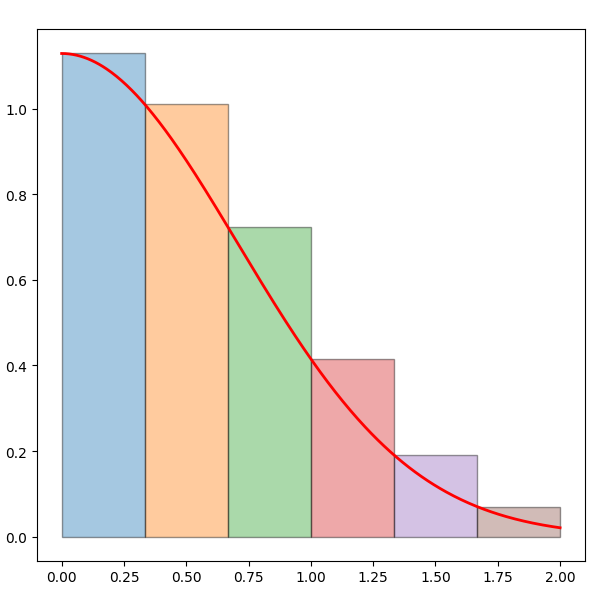
\includegraphics[width=0.7\textwidth]{img/left}
        \caption{Составная квадратурная формула левых прямоугольников с 6 разбиениями.}
        \label{fig:left}
    \end{figure}

    Обратим внимание на рисунок: проблема метода сразу становится очевидной --- в связи с монотонностью функции
    значительная часть прямоугольников выходит за подынтегральную функцию.
    Это и вызывает потребность в настолько больших количествах разбиений.

    \subsection{Метод центральных прямоугольников}\label{subsec:center}
    Определим значения функции~\eqref{eq:definition_erf}, применив составную квадратурную формулу метода центральных прямоугольников:
    \begin{equation}
        \label{eq:Quadrature_Formula_Centre_Rectangles}
        I_{N} = h \sum\limits_{i=1}^{N} f\left(\frac{x_i + x_{i-1}}{2}\right).
    \end{equation}
    Сравним полученные данные с результатами, рассчитанными с помощью ряда Тейлора.
    Итоги представлены в таблице~\ref{tab:Centre_Rectangles}.
    Возьмем в~\eqref{eq:Quadrature_Formula_Centre_Rectangles} количество разбиений~$N=6$.
    График этой формулы изображен на рис.~\ref{fig:Centre_Rectangles}.
    \begin{table}[H]
        \centering
        \begin{tabular}{|c|c|c|c|c|}
            \hline
            $x$  & $J_0(x)$ & $J_n(x)$ & $J_0(x)-J_n(x)$        & $n$ \\ \hline
            0.00 & 0.000000 & 0.000000 & 0                      & 1   \\ \hline
            0.20 & 0.222703 & 0.222703 & $1.79112\times10^{-7}$ & 64  \\ \hline
            0.40 & 0.428392 & 0.428393 & $3.13795\times10^{-7}$ & 128 \\ \hline
            0.60 & 0.603856 & 0.603856 & $2.09474\times10^{-7}$ & 256 \\ \hline
            0.80 & 0.742101 & 0.742101 & $1.31681\times10^{-7}$ & 512 \\ \hline
            1.00 & 0.842701 & 0.842701 & $1.45625\times10^{-7}$ & 512 \\ \hline
            1.20 & 0.910314 & 0.910314 & $7.35829\times10^{-8}$ & 512 \\ \hline
            1.40 & 0.952285 & 0.952285 & $8.63214\times10^{-8}$ & 512 \\ \hline
            1.60 & 0.976348 & 0.976348 & $6.21656\times10^{-8}$ & 512 \\ \hline
            1.80 & 0.989091 & 0.989091 & $2.6117\times10^{-7}$  & 256 \\ \hline
            2.00 & 0.995322 & 0.995322 & $1.00505\times10^{-7}$ & 256 \\ \hline
        \end{tabular}
        \caption{Результаты вычислений составной квадратурной формулой центральных прямоугольников.}
        \label{tab:Centre_Rectangles}
    \end{table}

    Этот метод обладает той же простотой, что и метод левых прямоугольников~\ref{subsec:left},
    однако на порядок более высокой точностью.
    Максимальное количество разбиений в этот раз составляет только $512$.

    \begin{figure}[H]
        \centering
        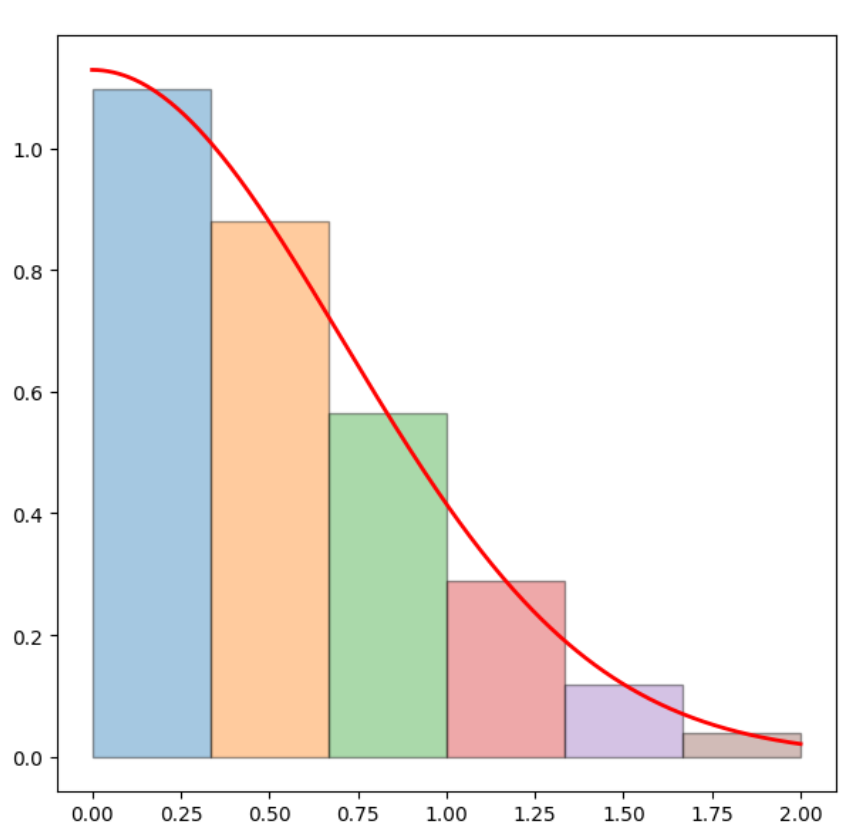
\includegraphics[width=0.7\textwidth]{img/center}
        \caption{Составная квадратурная формула центральных прямоугольников с 6 разбиениями.}
        \label{fig:Centre_Rectangles}
    \end{figure}

    Анализируя рисунок~\ref{fig:Centre_Rectangles} было сделано предположение,
    что преимущество над методом~\ref{subsec:left} заключается в первом и втором разбиении.
    Однако проверка показала: если для точек~$x=1,~x=n-1$ использовать метод центральных прямоугольников, то
    эффективность сильно страдает: приходится совершать до~$8\,388\,608$ разбиений.

    \subsection{Метод трапеций}\label{subsec:trapezoid}
    Рассчитаем~\eqref{eq:definition_erf}, применив составную квадратурную формулу метода трапеций:
    \begin{equation}
        \label{eq:Quadrature_Formula_Trapezoids}
        I_{N} = h \sum\limits_{i=1}^{N-1} \frac{f(x_i) + f(x_{i+1})}{2}.
    \end{equation}
    Сопоставим полученные данные с результатами, найденными с использованием ряда Тейлора.
    Все итоги записаны в таблицу~\ref{tab:Trapezoids}.
    Возьмем в~\eqref{eq:Quadrature_Formula_Trapezoids} количество разбиений~$N=6$.
    График этой формулы изображен на рис.~\ref{fig:Trapezoids}.
    \begin{table}[H]
        \centering
        \begin{tabular}{|c|c|c|c|c|}
            \hline
            $x$  & $J_0(x)$ & $J_n(x)$ & $J_0(x)-J_n(x)$        & $n$ \\ \hline
            0.00 & 0.000000 & 0.000000 & 0                      & 1   \\ \hline
            0.20 & 0.222703 & 0.222703 & $8.55699\times10^{-8}$ & 128 \\ \hline
            0.40 & 0.428392 & 0.428392 & $1.55708\times10^{-7}$ & 256 \\ \hline
            0.60 & 0.603856 & 0.603856 & $1.1486\times10^{-7}$  & 512 \\ \hline
            0.80 & 0.742101 & 0.742101 & $1.5884\times10^{-7}$  & 512 \\ \hline
            1.00 & 0.842701 & 0.842701 & $2.50252\times10^{-7}$ & 512 \\ \hline
            1.20 & 0.910314 & 0.910314 & $3.66987\times10^{-7}$ & 512 \\ \hline
            1.40 & 0.952285 & 0.952285 & $3.2961\times10^{-7}$  & 512 \\ \hline
            1.60 & 0.976348 & 0.976348 & $2.78573\times10^{-7}$ & 512 \\ \hline
            1.80 & 0.989091 & 0.989090 & $2.304\times10^{-7}$   & 512 \\ \hline
            2.00 & 0.995322 & 0.995322 & $2.14844\times10^{-7}$ & 512 \\ \hline
        \end{tabular}
        \caption{Результаты вычислений составной квадратурной формулой трапеций.}
        \label{tab:Trapezoids}
    \end{table}

    В этот раз максимальное количество необходимых разбиений не изменилось в сравнении с~\ref{subsec:center}
    и составило~$512$.
    Однако пик приходится на край отрезка разбиения $[0,2]$, в то время как
    в~\ref{subsec:center} он находился по центру.

    \begin{figure}[H]
        \centering
        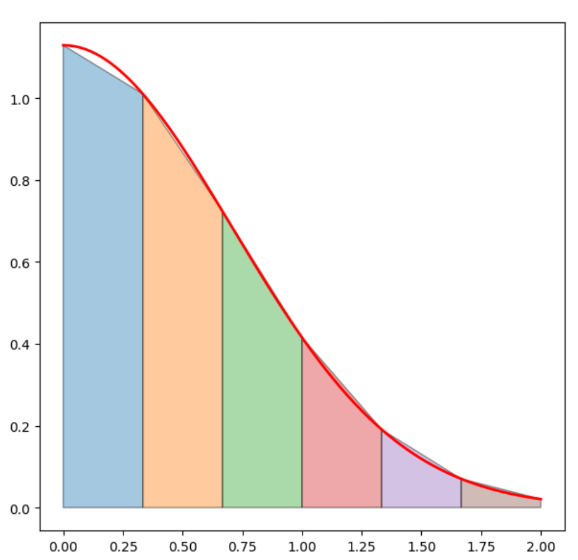
\includegraphics[width=0.7\textwidth]{img/trapezoid}
        \caption{Составная квадратурная формула трапеций с 6 разбиениями.}
        \label{fig:Trapezoids}
    \end{figure}

    \subsection{Метод Симпсона}\label{subsec:simpson}
    Построим квадратурную формулу Симпсона с тремя узлами
    $$ x_1=a, \qquad x_2=\frac{a+b}{2}, \qquad x_3=b, $$
    для вычисления интеграла
    $$ I = \int\limits_a^b f(x)dx. $$
    Параболу можно представить с помощью интерполяционного многочлена
    Лагранжа второй степени~$L_2(x)$ для функции~$f(x)$, который будет проходить через
    точки~$(x_1,f(x_1))$,~$(x_2,f(x_2))$,~$(x_3,f(x_3))$.
    Тогда интеграл приближенно равен:
    $$ I \approx \int\limits_a^b L_2(x)dx. $$
    Найденный интеграл можно представить с помощью весовых функций~$\omega_i$.
    $$ \int\limits_a^b L_2(x)dx = \omega_1 f(a) + \omega_2 f\left(\frac{a+b}{2}\right) + \omega_3 f(b). $$
    Благодаря симметрии узлов относительно центра отрезка, веса подчиняются
    равенству~$\omega_1 = \omega_3$, и при этом должно соблюдаться следующее:
    $$ \omega_1 + \omega_2 + \omega_3 = b-a. $$
    Вычислим веса~$\omega_i$ через интегралы от базисных функций:
    $$ \omega_2 = (b-a) \int\limits_0^1 \hat{l}_1(t) dt = (b-a) \int\limits_0^1 4t(1-t)dt = \frac{2}{3}(b-a). $$
    Тогда получаем, что
    $$ 2\omega_1 + \frac{2}{3}(b-a) = b-a \quad \Rightarrow \qquad \omega_1 = \omega_3 = \frac{b-a}{6}. $$
    Подставляя найденные веса, получаем формулу Симпсона:
    \begin{equation}
        \label{eq:Quadrature_Formula_Simpson}
        I \approx \frac{b-a}{6} \left(f(a) + 4 f\left(\frac{a+b}{2}\right) + f(b)\right).
    \end{equation}

    Вычислим, используя составную квадратурную формулу Симпсона:
    $$ I_{N} = \frac{h}{6} \sum\limits_{i=1}^{N-1} f(x_i) + 4 f\left(\frac{x_{i+1} + x_i}{2}\right) + f(x_{i+1}). $$
    Полученные данные сравним со значениями, вычисленными рядом Тейлора.
    Результаты занесены в таблицу~\ref{tab:Simpson}.
    График формулы~\eqref{eq:Quadrature_Formula_Simpson} изображен на рис.~\ref{fig:Simpson}.
    \begin{table}[H]
        \centering
        \begin{tabular}{|c|c|c|c|c|}
            \hline
            $x$  & $J_0(x)$ & $J_n(x)$ & $J_0(x)-J_n(x)$        & $n$ \\ \hline
            0.00 & 0.000000 & 0.000000 & 0                      & 1   \\ \hline
            0.20 & 0.222703 & 0.222703 & $8.15721\times10^{-9}$ & 4   \\ \hline
            0.40 & 0.428392 & 0.428392 & $9.74687\times10^{-9}$ & 8   \\ \hline
            0.60 & 0.603856 & 0.603856 & $4.06359\times10^{-8}$ & 8   \\ \hline
            0.80 & 0.742101 & 0.742101 & $4.19496\times10^{-8}$ & 16  \\ \hline
            1.00 & 0.842701 & 0.842701 & $2.24613\times10^{-8}$ & 16  \\ \hline
            1.20 & 0.910314 & 0.910314 & $4.78853\times10^{-8}$ & 8   \\ \hline
            1.40 & 0.952285 & 0.952285 & $6.90624\times10^{-8}$ & 16  \\ \hline
            1.60 & 0.976348 & 0.976348 & $9.26237\times10^{-8}$ & 16  \\ \hline
            1.80 & 0.989091 & 0.989090 & $1.28231\times10^{-7}$ & 16  \\ \hline
            2.00 & 0.995322 & 0.995322 & $1.14107\times10^{-7}$ & 32  \\ \hline
        \end{tabular}
        \caption{Результаты вычислений составной квадратурной формулой Симпсона.}
        \label{tab:Simpson}
    \end{table}

    Полученный результат можно назвать серьезным --- потребовалось сделать не более $32$ разбиений для удовлетворения
    необходимой точности.
    Логика алгоритма стала сложнее, что компенсируется на порядок более высокой скоростью.

    \begin{figure}[H]
        \centering
        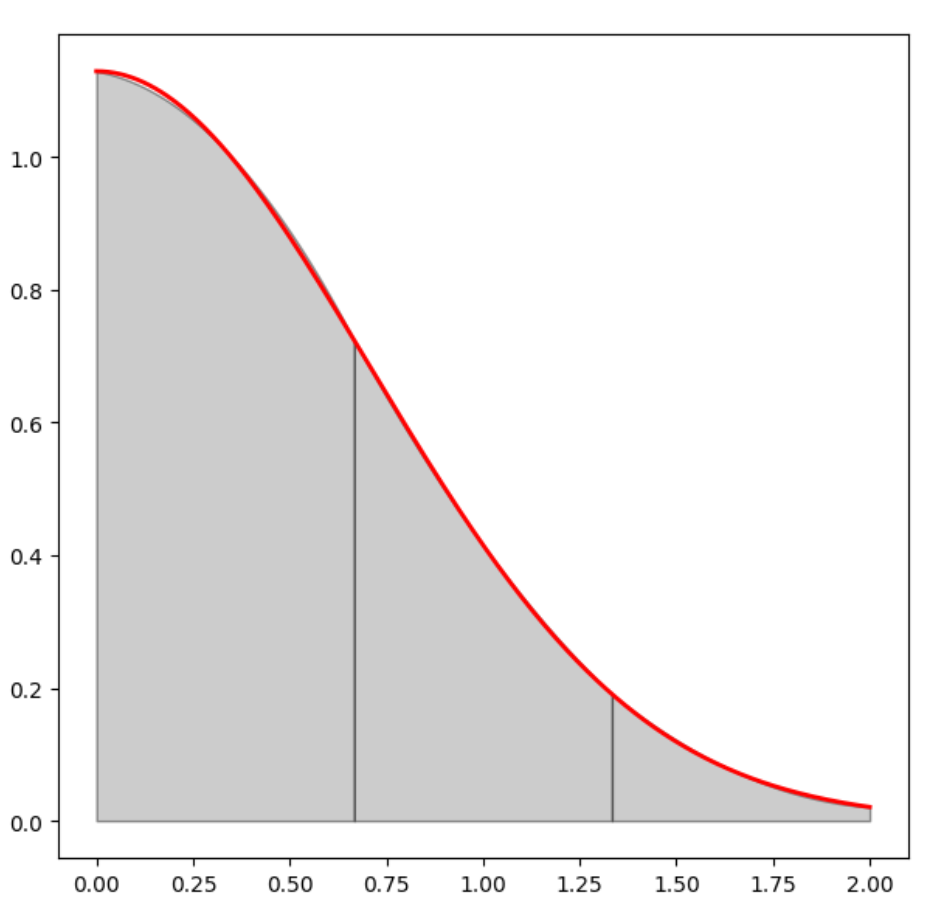
\includegraphics[width=0.7\textwidth]{img/simpson}
        \caption{Квадратурная формула Симпсона c 3 разбиениями.}
        \label{fig:Simpson}
    \end{figure}

    На рисунке~\ref{fig:Simpson} видно, что сплайн из 3 парабол уже практически полностью
    покрывает площадь под графиком.

    \subsection{Метод Гаусса}\label{subsec:gaussian}
    Вычислим~\eqref{eq:definition_erf}, используя составную квадратурную формулу Гаусса:
    \begin{equation}
        \label{eq:Quadrature_Formula_Gauss}
        I_{N} = \frac{h}{2} \sum\limits_{i=1}^{N-1} f\left(x_i + \frac{h}{2}\left(1 - \frac{1}{\sqrt{3}}\right)\right) + f\left(x_i + \frac{h}{2}\left(1 + \frac{1}{\sqrt{3}}\right)\right).
    \end{equation}
    Сравним полученные результаты с данными, рассчитанными с использованием ряда Тейлора.
    Все итоги отражены в таблице~\ref{tab:Gauss}.
    \begin{table}[H]
        \centering
        \begin{tabular}{|c|c|c|c|c|}
            \hline
            $x$  & $J_0(x)$ & $J_n(x)$ & $J_0(x)-J_n(x)$        & $n$ \\ \hline
            0.00 & 0.000000 & 0.000000 & 0                      & 1   \\ \hline
            0.20 & 0.222703 & 0.222703 & $5.61481\times10^{-8}$ & 2   \\ \hline
            0.40 & 0.428392 & 0.428392 & $5.17605\times10^{-9}$ & 8   \\ \hline
            0.60 & 0.603856 & 0.603856 & $3.83412\times10^{-8}$ & 8   \\ \hline
            0.80 & 0.742101 & 0.742101 & $3.01009\times10^{-8}$ & 16  \\ \hline
            1.00 & 0.842701 & 0.842701 & $7.80269\times10^{-9}$ & 16  \\ \hline
            1.20 & 0.910314 & 0.910314 & $9.01245\times10^{-8}$ & 8   \\ \hline
            1.40 & 0.952285 & 0.952285 & $4.11593\times10^{-8}$ & 16  \\ \hline
            1.60 & 0.976348 & 0.976348 & $2.39354\times10^{-8}$ & 16  \\ \hline
            1.80 & 0.989091 & 0.989091 & $2.54125\times10^{-8}$ & 16  \\ \hline
            2.00 & 0.995322 & 0.995322 & $6.29995\times10^{-8}$ & 16  \\ \hline
        \end{tabular}
        \caption{Результаты вычислений составной квадратурной формулой Гаусса.}
        \label{tab:Gauss}
    \end{table}

    Самый эффективный метод.
    При фактически эквивалентной сложности алгоритма методу~\ref{subsec:simpson} необходимое количество разбиений
    уменьшилось вдвое и не превысило~$16$.
    Однако концепция метода намного сложнее чем рассмотренные выше --- это не попытка замощения площади под графиком
    другими функциями, поэтому попытка изобразить процесс графически лишена своего смысла.
    \newpage


    \section{Вывод}\label{sec:}
    В процессе исследования были реализованы и протестированы 5 квадратурных методов.
    Был проведен анализ и избран самый эффективный из них.

    Метод левых прямоугольников оказался самым бесполезным: с аналогичной сложностью лучше избирать метод центральных
    прямоугольников, который лучше во всем.
    Тем не менее он все так же мало эффективен.
    Метод трапеций не показал лучших результатов, чем метод центральных прямоугольников.

    Пускай число разбиений $N=512$ и является предпочтительнее $2\,097\,152$, они все еще проигрывают двум самым
    эффективным методам --- Гаусса и Симпсона.
    Первый оказался в 2 раза эффективней второго.
    Ошибка метода Симсона оказалась несколько меньше.
    Однако это преимущество сомнительно, поскольку метод Гаусса является более быстрым, из-за чего при желании
    можно добиться даже большой точности, если увеличить число разбиений.
    \newpage

    \section{Листинг программы}
    {\small
        \begin{verbatim}
            #pragma once
            #include <complex>
            #include <functional>

            namespace integral_methods {
            constexpr static double GAUSSIAN_FACTOR_L = 1 - 1/std::sqrt(3);
            constexpr static double GAUSSIAN_FACTOR_G = 1 + 1/std::sqrt(3);

            inline double calculate_left_integral(
                std::vector<double> dots, const std::function<double(double)> &f)
            {
                double result = 0;
                for (int i = 0; i < dots.size() - 1; i++) {
                    result += (dots[i + 1] - dots[i]) * f(dots[i]);
                }

                return result;
            }

            inline double calculate_right_integral(
                std::vector<double> dots, const std::function<double(double)> &f)
            {
                double result = 0;
                for (int i = 1; i < dots.size(); i++) {
                    result += (dots[i + 1] - dots[i]) * f(dots[i + 1]);
                }

                return result;
            }

            inline double calculate_central_integral(
                std::vector<double> dots, const std::function<double(double)> &f)
            {
                double result = 0;
                for (int i = 0; i < dots.size() - 1; i++) {
                    auto left = dots[i];
                    auto right = dots[i + 1];
                    auto central = (left + right) / 2;

                    result += (right - left) * f(central);
                }

                return result;
            }

            inline double calculate_trapezoid_integral(
                std::vector<double> dots, const std::function<double(double)> &f)
            {
                double result = 0;
                for (int i = 0; i < dots.size() - 1; i++) {
                    auto left = dots[i];
                    auto right = dots[i + 1];

                    result += (right - left) * (f(left) + f(right)) / 2;
                }

                return result;
            }

            inline double calculate_simpson_integral(
                std::vector<double> dots, const std::function<double(double)> &f)
            {
                double result = 0;
                for (int i = 0; i < dots.size() - 1; i++) {
                    auto left = dots[i];
                    auto right = dots[i + 1];
                    auto f_factor = f(left) + 4 * f((left + right) / 2) + f(right);

                    result += (right - left) / 6 * f_factor;
                }

                return result;
            }

            inline double calculate_gaussian_integral(
                std::vector<double> dots, const std::function<double(double)> &f)
            {
                double result = 0;

                for (int i = 0; i < dots.size() - 1; i++) {
                    auto left = dots[i];
                    auto right = dots[i + 1];
                    auto h_half = (right - left) / 2;
                    auto f_factor = f(left + h_half * GAUSSIAN_FACTOR_L)
                                    + f(left + h_half * GAUSSIAN_FACTOR_G);

                    result += h_half * f_factor;
                }

                return result;
            }
            } // namespace integral_methods
        \end{verbatim}
    }\label{sec:-3}
\end{document}